\section{Controlled ablations, adaptation and transfer}\label{sec:section-07}

R5-momentum: candidate-minus-reference log loss -0.0022 (lower loss), 95\% interval [-0.0099, 0.0057], Holm p=1.000. R5-trend: candidate-minus-reference log loss 0.0027 (higher loss), 95\% interval [-0.0020, 0.0075], Holm p=1.000. R5-risk: candidate-minus-reference log loss -0.0021 (lower loss), 95\% interval [-0.0097, 0.0054], Holm p=1.000. R5-context\_volume: candidate-minus-reference log loss 0.0053 (higher loss), 95\% interval [0.0005, 0.0100], Holm p=0.243.

\noindent Table~\ref{tab:8} reports controlled feature ablations.

\begin{table}[!htbp]\centering\footnotesize\setlength{\tabcolsep}{3pt}\renewcommand{\arraystretch}{1.14}
\caption{Controlled feature ablations}\label{tab:8}
\begin{tabular}{@{}>{\raggedright\arraybackslash}p{\dimexpr 0.25758\textwidth-5.000pt\relax}>{\raggedleft\arraybackslash}p{\dimexpr 0.14773\textwidth-5.000pt\relax}>{\raggedleft\arraybackslash}p{\dimexpr 0.15152\textwidth-5.000pt\relax}>{\raggedleft\arraybackslash}p{\dimexpr 0.14773\textwidth-5.000pt\relax}>{\raggedleft\arraybackslash}p{\dimexpr 0.14773\textwidth-5.000pt\relax}>{\raggedleft\arraybackslash}p{\dimexpr 0.14773\textwidth-5.000pt\relax}@{}}
\toprule
\textbf{Contrast} & \textbf{Rows} & \textbf{Loss delta} & \textbf{CI low} & \textbf{CI high} & \textbf{Holm p} \\
\midrule
R5-momentum & 5,544 & -0.0022 & -0.0099 & 0.0057 & 1.000 \\
R5-trend & 5,544 & 0.0027 & -0.0020 & 0.0075 & 1.000 \\
R5-risk & 5,544 & -0.0021 & -0.0097 & 0.0054 & 1.000 \\
R5-context\_\allowbreak{}volume & 5,544 & 0.0053 & 0.0005 & 0.0100 & 0.243 \\
\bottomrule\end{tabular}\par\smallskip
\raggedright\textit{Source:} \path{data/research-v2/tables/exp_contrasts.csv}.
\end{table}


\noindent Figure~\ref{fig:7} shows registered controlled contrasts on development outer blocks; intervals preserve date dependence.

\begin{figure}[htbp]\centering
% Native editable figure; frozen statistics 0d291b4aebf8c524dc6705d872c070feb990e86a1cebbd59a758f400b240c952
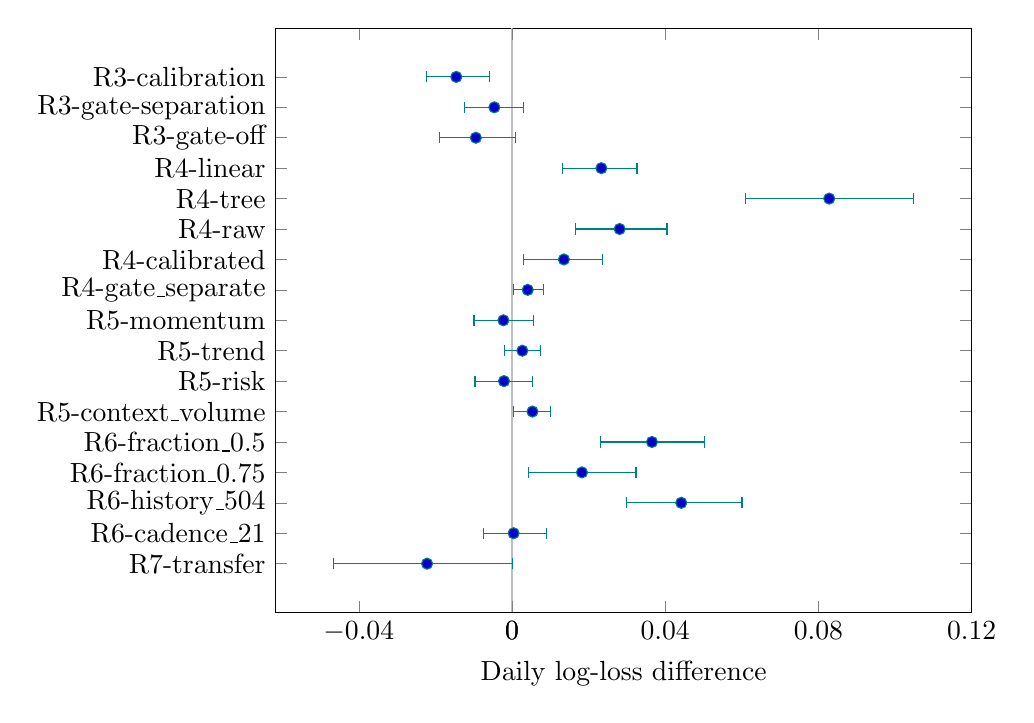
\begin{tikzpicture}
\begin{axis}[width=.86\linewidth,height=9cm,ytick={0,1,2,3,4,5,6,7,8,9,10,11,12,13,14,15,16},yticklabels={{R7-transfer},{R6-cadence\_21},{R6-history\_504},{R6-fraction\_0.75},{R6-fraction\_0.5},{R5-context\_volume},{R5-risk},{R5-trend},{R5-momentum},{R4-gate\_separate},{R4-calibrated},{R4-raw},{R4-tree},{R4-linear},{R3-gate-off},{R3-gate-separation},{R3-calibration}},xlabel={Daily log-loss difference},scaled x ticks=false,xtick={-.04,0,.04,.08,.12},x tick label style={/pgf/number format/fixed,/pgf/number format/precision=2},extra x ticks={0},extra x tick style={grid=major}]
\addplot+[teal,only marks,mark=*,error bars/.cd,x dir=both,x explicit] table[x=x,y=y,x error minus=lo,x error plus=hi,row sep=\\]{x y lo hi\\-0.0221801343161 0 0.024455579808 0.0223931852201\\
0.00041632232384 1 0.00791390874367 0.00868206037013\\
0.0441811010945 2 0.0143275954856 0.015861729419\\
0.0182631117218 3 0.0138705225454 0.0141196775605\\
0.0365366597573 4 0.0133799431661 0.0137957905223\\
0.00533639532695 5 0.00486071784276 0.00466252994581\\
-0.00209736606647 6 0.00755715195286 0.00749668667262\\
0.00269779404642 7 0.00471778582188 0.00481513474751\\
-0.00224943558219 8 0.00768731950008 0.00793827176469\\
0.00410115278394 9 0.00372147435029 0.00402768313738\\
0.0135461882894 10 0.0104981010291 0.0101189671534\\
0.028097358561 11 0.0115527059594 0.0123625312577\\
0.0828103310099 12 0.0219448112081 0.0220977857158\\
0.0233234605807 13 0.0100885775788 0.00930814049429\\
-0.00944503550542 14 0.00953611262778 0.0104141759139\\
-0.00461796099919 15 0.00779347490533 0.00755609905958\\
-0.0145511702716 16 0.00775600532129 0.00857025671815\\};

\end{axis}
\end{tikzpicture}

\caption{Registered controlled contrasts on development outer blocks; intervals preserve date dependence.}\label{fig:7}
\end{figure}

A feature-importance ranking is not a feature ablation. The experiments remove a registered feature family, refit the eligible model and compare outer predictions on matching dates. This evaluates the value of allowing that family under the stated model and budget. Correlated families can substitute for one another; removing one does not estimate an isolated economic causal effect. The sign of an ablation also depends on regularization and sampling variance. We retain unfavorable and near-zero changes alongside any improvement.

R3-calibration: candidate-minus-reference log loss -0.0146 (lower loss), 95\% interval [-0.0223, -0.0060], Holm p=0.018. R3-gate-separation: candidate-minus-reference log loss -0.0046 (lower loss), 95\% interval [-0.0124, 0.0029], Holm p=1.000. R3-gate-off: candidate-minus-reference log loss -0.0094 (lower loss), 95\% interval [-0.0190, 0.0010], Holm p=0.458. The forecast gate here chooses between calibrated predictions and the prior as a diagnostic view. The portfolio gate separately controls the trend/ML weight. Neither is silently substituted for the frozen trend shadow.

\noindent Table~\ref{tab:9} reports controlled base forecast views on development outer blocks.

\begin{table}[!htbp]\centering\footnotesize\setlength{\tabcolsep}{3pt}\renewcommand{\arraystretch}{1.14}
\caption{Controlled base forecast views on development outer blocks}\label{tab:9}
\begin{tabular}{@{}>{\raggedright\arraybackslash}p{\dimexpr 0.20000\textwidth-5.000pt\relax}>{\raggedleft\arraybackslash}p{\dimexpr 0.15000\textwidth-5.000pt\relax}>{\raggedleft\arraybackslash}p{\dimexpr 0.15000\textwidth-5.000pt\relax}>{\raggedleft\arraybackslash}p{\dimexpr 0.15000\textwidth-5.000pt\relax}>{\raggedleft\arraybackslash}p{\dimexpr 0.15000\textwidth-5.000pt\relax}>{\raggedleft\arraybackslash}p{\dimexpr 0.20000\textwidth-5.000pt\relax}@{}}
\toprule
\textbf{View} & \textbf{Rows} & \textbf{Accuracy} & \textbf{Log loss} & \textbf{Brier} & \textbf{Separate gate} \\
\midrule
calibrated & 5,544 & 40.13\% & 1.0773 & 0.6549 & 27.27\% \\
gate\_\allowbreak{}same & 5,544 & 42.14\% & 1.0725 & 0.6516 & 27.27\% \\
gate\_\allowbreak{}separate & 5,544 & 41.94\% & 1.0679 & 0.6482 & 27.27\% \\
linear & 5,544 & 39.30\% & 1.0871 & 0.6628 & 27.27\% \\
prior & 5,544 & 42.19\% & 1.0638 & 0.6453 & 27.27\% \\
raw & 5,544 & 40.13\% & 1.0919 & 0.6657 & 27.27\% \\
tree & 5,544 & 40.22\% & 1.1466 & 0.6971 & 27.27\% \\
\bottomrule\end{tabular}\par\smallskip
\raggedright\textit{Source:} \path{data/research-v2/tables/exp_predictive.csv}.
\end{table}


R6-fraction\_0.5: candidate-minus-reference log loss 0.0365 (higher loss), 95\% interval [0.0232, 0.0503], Holm p=0.008. R6-fraction\_0.75: candidate-minus-reference log loss 0.0183 (higher loss), 95\% interval [0.0044, 0.0324], Holm p=0.082. R6-history\_504: candidate-minus-reference log loss 0.0442 (higher loss), 95\% interval [0.0299, 0.0600], Holm p=0.008. R6-cadence\_21: candidate-minus-reference log loss 0.0004 (higher loss), 95\% interval [-0.0075, 0.0091], Holm p=1.000.

\noindent Table~\ref{tab:10} reports controlled history, fraction and cadence contrasts.

\begin{table}[!htbp]\centering\footnotesize\setlength{\tabcolsep}{3pt}\renewcommand{\arraystretch}{1.14}
\caption{Controlled history, fraction and cadence contrasts}\label{tab:10}
\begin{tabular}{@{}>{\raggedright\arraybackslash}p{\dimexpr 0.24615\textwidth-5.000pt\relax}>{\raggedleft\arraybackslash}p{\dimexpr 0.15000\textwidth-5.000pt\relax}>{\raggedleft\arraybackslash}p{\dimexpr 0.15385\textwidth-5.000pt\relax}>{\raggedleft\arraybackslash}p{\dimexpr 0.15000\textwidth-5.000pt\relax}>{\raggedleft\arraybackslash}p{\dimexpr 0.15000\textwidth-5.000pt\relax}>{\raggedleft\arraybackslash}p{\dimexpr 0.15000\textwidth-5.000pt\relax}@{}}
\toprule
\textbf{Contrast} & \textbf{Rows} & \textbf{Loss delta} & \textbf{CI low} & \textbf{CI high} & \textbf{Holm p} \\
\midrule
R6-fraction\_\allowbreak{}0.5 & 5,544 & 0.0365 & 0.0232 & 0.0503 & 0.008 \\
R6-fraction\_\allowbreak{}0.75 & 5,544 & 0.0183 & 0.0044 & 0.0324 & 0.082 \\
R6-history\_\allowbreak{}504 & 5,544 & 0.0442 & 0.0299 & 0.0600 & 0.008 \\
R6-cadence\_\allowbreak{}21 & 1,512 & 0.0004 & -0.0075 & 0.0091 & 1.000 \\
\bottomrule\end{tabular}\par\smallskip
\raggedright\textit{Source:} \path{data/research-v2/tables/exp_contrasts.csv}.
\end{table}


\noindent Figure~\ref{fig:8} shows fitting versus outer validation log loss under training-design changes.

\begin{figure}[htbp]\centering
% Native editable figure; frozen statistics 0d291b4aebf8c524dc6705d872c070feb990e86a1cebbd59a758f400b240c952
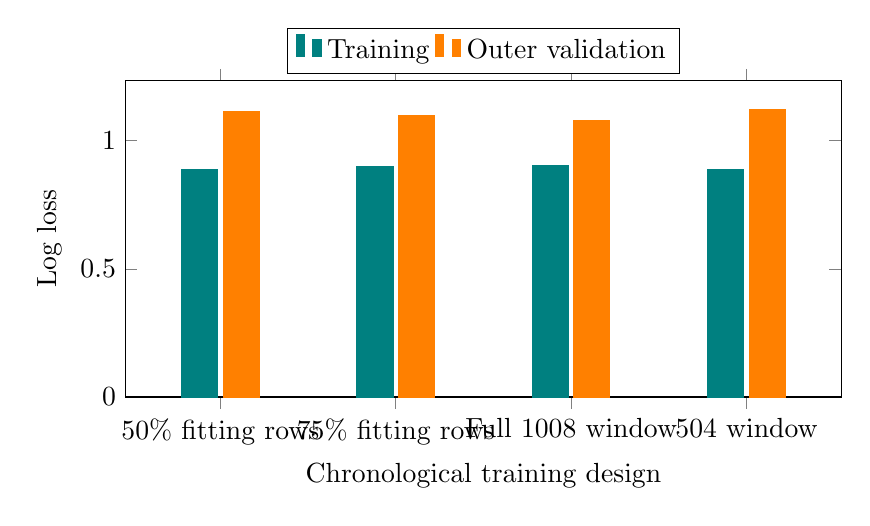
\begin{tikzpicture}
\begin{axis}[width=.88\linewidth,height=5.6cm,ybar,bar width=13pt,ymin=0,xtick={0,1,2,3},xticklabels={50\% fitting rows,75\% fitting rows,Full 1008 window,504 window},xlabel={Chronological training design},ylabel={Log loss},legend columns=2,legend style={at={(.5,1.02)},anchor=south},enlarge x limits=.18]
\addplot+[teal] coordinates {(0,0.885257437617) (1,0.899655741498) (2,0.904358782174) (3,0.887661478304)};
\addlegendentry{Training}
\addplot+[orange] coordinates {(0,1.11388215622) (1,1.09560860818) (2,1.07734549646) (3,1.12152659756)};
\addlegendentry{Outer validation}

\end{axis}
\end{tikzpicture}

\caption{Fitting versus outer validation log loss under training-design changes.}\label{fig:8}
\end{figure}

Across the registered seed comparisons, the largest probability difference is 0.0e+00. The tested deterministic estimator settings therefore produced identical probabilities across seeds. Zero seed variation is not zero research uncertainty: the calendar path, data vintage, history span and target instrument remain sources of variation. Shorter recent-history fractions change both row count and temporal span, so the learning curves do not identify a pure sample-size effect. Separating the gate also changes its recency as well as its information overlap.

Learning curves report fitting and outer-period loss together. A widening gap can be consistent with variance or time shift, while high loss on both partitions can indicate limited representation or model capacity. A smaller history can adapt faster but discard rare conditions; a larger history can stabilize estimation while retaining outdated relationships. Refit-cadence tests ask whether refreshing a fixed model matters under aligned information. No cadence is promoted merely because it is best on these consumed development blocks.

R7-transfer: candidate-minus-reference log loss -0.0222 (lower loss), 95\% interval [-0.0466, 0.0002], Holm p=0.458. The held-target comparison reports the aligned target subset only. Training on other instruments increases the number of fitting rows but does not increase the number of independent outer dates.

\noindent Table~\ref{tab:11} reports controlled held-instrument transfer contrast.

\begin{table}[!htbp]\centering\footnotesize\setlength{\tabcolsep}{3pt}\renewcommand{\arraystretch}{1.14}
\caption{Controlled held-instrument transfer contrast}\label{tab:11}
\begin{tabular}{@{}>{\raggedright\arraybackslash}p{\dimexpr 0.18333\textwidth-5.000pt\relax}>{\raggedleft\arraybackslash}p{\dimexpr 0.16250\textwidth-5.000pt\relax}>{\raggedleft\arraybackslash}p{\dimexpr 0.16667\textwidth-5.000pt\relax}>{\raggedleft\arraybackslash}p{\dimexpr 0.16250\textwidth-5.000pt\relax}>{\raggedleft\arraybackslash}p{\dimexpr 0.16250\textwidth-5.000pt\relax}>{\raggedleft\arraybackslash}p{\dimexpr 0.16250\textwidth-5.000pt\relax}@{}}
\toprule
\textbf{Contrast} & \textbf{Rows} & \textbf{Loss delta} & \textbf{CI low} & \textbf{CI high} & \textbf{Holm p} \\
\midrule
R7-transfer & 1,512 & -0.0222 & -0.0466 & 0.0002 & 0.458 \\
\bottomrule\end{tabular}\par\smallskip
\raggedright\textit{Source:} \path{data/research-v2/tables/exp_contrasts.csv}.
\end{table}


\noindent Figure~\ref{fig:9} shows historical instrument/period heterogeneity. Consumed-period slices are descriptive.

\begin{figure}[htbp]\centering
% Native editable figure; frozen statistics 0d291b4aebf8c524dc6705d872c070feb990e86a1cebbd59a758f400b240c952
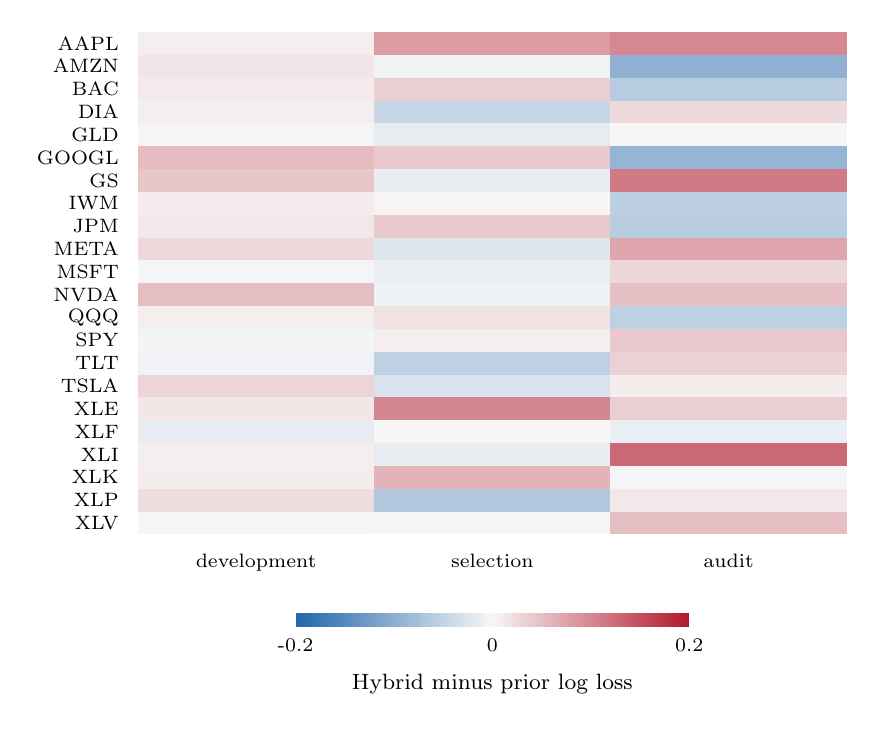
\begin{tikzpicture}[x=1cm,y=1cm,font=\scriptsize]
\node[anchor=east] at (-.12,6.235) {AAPL};
\fill[fill={rgb,255:red,244;green,238;blue,239}] (0,6.09) rectangle ++(3,0.29);
\fill[fill={rgb,255:red,219;green,156;blue,164}] (3,6.09) rectangle ++(3,0.29);
\fill[fill={rgb,255:red,213;green,136;blue,146}] (6,6.09) rectangle ++(3,0.29);
\node[anchor=east] at (-.12,5.945) {AMZN};
\fill[fill={rgb,255:red,241;green,229;blue,231}] (0,5.8) rectangle ++(3,0.29);
\fill[fill={rgb,255:red,242;green,243;blue,245}] (3,5.8) rectangle ++(3,0.29);
\fill[fill={rgb,255:red,144;green,177;blue,211}] (6,5.8) rectangle ++(3,0.29);
\node[anchor=east] at (-.12,5.655) {BAC};
\fill[fill={rgb,255:red,243;green,234;blue,235}] (0,5.51) rectangle ++(3,0.29);
\fill[fill={rgb,255:red,235;green,208;blue,211}] (3,5.51) rectangle ++(3,0.29);
\fill[fill={rgb,255:red,184;green,204;blue,225}] (6,5.51) rectangle ++(3,0.29);
\node[anchor=east] at (-.12,5.365) {DIA};
\fill[fill={rgb,255:red,244;green,238;blue,239}] (0,5.22) rectangle ++(3,0.29);
\fill[fill={rgb,255:red,198;green,214;blue,230}] (3,5.22) rectangle ++(3,0.29);
\fill[fill={rgb,255:red,238;green,218;blue,220}] (6,5.22) rectangle ++(3,0.29);
\node[anchor=east] at (-.12,5.075) {GLD};
\fill[fill={rgb,255:red,246;green,245;blue,245}] (0,4.93) rectangle ++(3,0.29);
\fill[fill={rgb,255:red,231;green,236;blue,241}] (3,4.93) rectangle ++(3,0.29);
\fill[fill={rgb,255:red,246;green,246;blue,246}] (6,4.93) rectangle ++(3,0.29);
\node[anchor=east] at (-.12,4.785) {GOOGL};
\fill[fill={rgb,255:red,229;green,188;blue,193}] (0,4.64) rectangle ++(3,0.29);
\fill[fill={rgb,255:red,233;green,201;blue,205}] (3,4.64) rectangle ++(3,0.29);
\fill[fill={rgb,255:red,150;green,181;blue,213}] (6,4.64) rectangle ++(3,0.29);
\node[anchor=east] at (-.12,4.495) {GS};
\fill[fill={rgb,255:red,232;green,199;blue,203}] (0,4.35) rectangle ++(3,0.29);
\fill[fill={rgb,255:red,233;green,237;blue,242}] (3,4.35) rectangle ++(3,0.29);
\fill[fill={rgb,255:red,208;green,122;blue,133}] (6,4.35) rectangle ++(3,0.29);
\node[anchor=east] at (-.12,4.205) {IWM};
\fill[fill={rgb,255:red,244;green,236;blue,237}] (0,4.06) rectangle ++(3,0.29);
\fill[fill={rgb,255:red,246;green,244;blue,244}] (3,4.06) rectangle ++(3,0.29);
\fill[fill={rgb,255:red,189;green,208;blue,227}] (6,4.06) rectangle ++(3,0.29);
\node[anchor=east] at (-.12,3.915) {JPM};
\fill[fill={rgb,255:red,242;green,232;blue,234}] (0,3.77) rectangle ++(3,0.29);
\fill[fill={rgb,255:red,233;green,201;blue,205}] (3,3.77) rectangle ++(3,0.29);
\fill[fill={rgb,255:red,185;green,205;blue,225}] (6,3.77) rectangle ++(3,0.29);
\node[anchor=east] at (-.12,3.625) {META};
\fill[fill={rgb,255:red,238;green,216;blue,219}] (0,3.48) rectangle ++(3,0.29);
\fill[fill={rgb,255:red,222;green,230;blue,238}] (3,3.48) rectangle ++(3,0.29);
\fill[fill={rgb,255:red,222;green,165;blue,172}] (6,3.48) rectangle ++(3,0.29);
\node[anchor=east] at (-.12,3.335) {MSFT};
\fill[fill={rgb,255:red,244;green,245;blue,246}] (0,3.19) rectangle ++(3,0.29);
\fill[fill={rgb,255:red,234;green,238;blue,242}] (3,3.19) rectangle ++(3,0.29);
\fill[fill={rgb,255:red,237;green,214;blue,217}] (6,3.19) rectangle ++(3,0.29);
\node[anchor=east] at (-.12,3.045) {NVDA};
\fill[fill={rgb,255:red,229;green,190;blue,195}] (0,2.9) rectangle ++(3,0.29);
\fill[fill={rgb,255:red,239;green,242;blue,244}] (3,2.9) rectangle ++(3,0.29);
\fill[fill={rgb,255:red,230;green,192;blue,196}] (6,2.9) rectangle ++(3,0.29);
\node[anchor=east] at (-.12,2.755) {QQQ};
\fill[fill={rgb,255:red,244;green,238;blue,239}] (0,2.61) rectangle ++(3,0.29);
\fill[fill={rgb,255:red,240;green,225;blue,226}] (3,2.61) rectangle ++(3,0.29);
\fill[fill={rgb,255:red,190;green,209;blue,227}] (6,2.61) rectangle ++(3,0.29);
\node[anchor=east] at (-.12,2.465) {SPY};
\fill[fill={rgb,255:red,242;green,244;blue,245}] (0,2.32) rectangle ++(3,0.29);
\fill[fill={rgb,255:red,244;green,238;blue,239}] (3,2.32) rectangle ++(3,0.29);
\fill[fill={rgb,255:red,232;green,200;blue,204}] (6,2.32) rectangle ++(3,0.29);
\node[anchor=east] at (-.12,2.175) {TLT};
\fill[fill={rgb,255:red,240;green,242;blue,245}] (0,2.03) rectangle ++(3,0.29);
\fill[fill={rgb,255:red,190;green,209;blue,227}] (3,2.03) rectangle ++(3,0.29);
\fill[fill={rgb,255:red,235;green,208;blue,212}] (6,2.03) rectangle ++(3,0.29);
\node[anchor=east] at (-.12,1.885) {TSLA};
\fill[fill={rgb,255:red,236;green,212;blue,215}] (0,1.74) rectangle ++(3,0.29);
\fill[fill={rgb,255:red,218;green,227;blue,237}] (3,1.74) rectangle ++(3,0.29);
\fill[fill={rgb,255:red,244;green,236;blue,237}] (6,1.74) rectangle ++(3,0.29);
\node[anchor=east] at (-.12,1.595) {XLE};
\fill[fill={rgb,255:red,242;green,230;blue,231}] (0,1.45) rectangle ++(3,0.29);
\fill[fill={rgb,255:red,212;green,134;blue,144}] (3,1.45) rectangle ++(3,0.29);
\fill[fill={rgb,255:red,234;green,206;blue,209}] (6,1.45) rectangle ++(3,0.29);
\node[anchor=east] at (-.12,1.305) {XLF};
\fill[fill={rgb,255:red,231;green,236;blue,241}] (0,1.16) rectangle ++(3,0.29);
\fill[fill={rgb,255:red,247;green,246;blue,246}] (3,1.16) rectangle ++(3,0.29);
\fill[fill={rgb,255:red,233;green,238;blue,242}] (6,1.16) rectangle ++(3,0.29);
\node[anchor=east] at (-.12,1.015) {XLI};
\fill[fill={rgb,255:red,244;green,238;blue,239}] (0,0.87) rectangle ++(3,0.29);
\fill[fill={rgb,255:red,232;green,237;blue,242}] (3,0.87) rectangle ++(3,0.29);
\fill[fill={rgb,255:red,203;green,104;blue,117}] (6,0.87) rectangle ++(3,0.29);
\node[anchor=east] at (-.12,0.725) {XLK};
\fill[fill={rgb,255:red,244;green,236;blue,237}] (0,0.58) rectangle ++(3,0.29);
\fill[fill={rgb,255:red,226;green,180;blue,186}] (3,0.58) rectangle ++(3,0.29);
\fill[fill={rgb,255:red,243;green,245;blue,246}] (6,0.58) rectangle ++(3,0.29);
\node[anchor=east] at (-.12,0.435) {XLP};
\fill[fill={rgb,255:red,239;green,220;blue,223}] (0,0.29) rectangle ++(3,0.29);
\fill[fill={rgb,255:red,177;green,200;blue,223}] (3,0.29) rectangle ++(3,0.29);
\fill[fill={rgb,255:red,242;green,231;blue,233}] (6,0.29) rectangle ++(3,0.29);
\node[anchor=east] at (-.12,0.145) {XLV};
\fill[fill={rgb,255:red,243;green,245;blue,246}] (0,0) rectangle ++(3,0.29);
\fill[fill={rgb,255:red,246;green,246;blue,246}] (3,0) rectangle ++(3,0.29);
\fill[fill={rgb,255:red,230;green,191;blue,196}] (6,0) rectangle ++(3,0.29);
\node[anchor=north,align=center] at (1.5,-.12) {development};
\node[anchor=north,align=center] at (4.5,-.12) {selection};
\node[anchor=north,align=center] at (7.5,-.12) {audit};
\fill[fill={rgb,255:red,35;green,103;blue,173}] (2,-1.18) rectangle ++(.051,.18);
\fill[fill={rgb,255:red,39;green,106;blue,174}] (2.05,-1.18) rectangle ++(.051,.18);
\fill[fill={rgb,255:red,44;green,109;blue,176}] (2.1,-1.18) rectangle ++(.051,.18);
\fill[fill={rgb,255:red,48;green,112;blue,177}] (2.15,-1.18) rectangle ++(.051,.18);
\fill[fill={rgb,255:red,52;green,115;blue,179}] (2.2,-1.18) rectangle ++(.051,.18);
\fill[fill={rgb,255:red,57;green,118;blue,180}] (2.25,-1.18) rectangle ++(.051,.18);
\fill[fill={rgb,255:red,61;green,121;blue,182}] (2.3,-1.18) rectangle ++(.051,.18);
\fill[fill={rgb,255:red,65;green,124;blue,183}] (2.35,-1.18) rectangle ++(.051,.18);
\fill[fill={rgb,255:red,69;green,127;blue,185}] (2.4,-1.18) rectangle ++(.051,.18);
\fill[fill={rgb,255:red,74;green,130;blue,186}] (2.45,-1.18) rectangle ++(.051,.18);
\fill[fill={rgb,255:red,78;green,132;blue,188}] (2.5,-1.18) rectangle ++(.051,.18);
\fill[fill={rgb,255:red,82;green,135;blue,189}] (2.55,-1.18) rectangle ++(.051,.18);
\fill[fill={rgb,255:red,86;green,138;blue,191}] (2.6,-1.18) rectangle ++(.051,.18);
\fill[fill={rgb,255:red,91;green,141;blue,192}] (2.65,-1.18) rectangle ++(.051,.18);
\fill[fill={rgb,255:red,95;green,144;blue,194}] (2.7,-1.18) rectangle ++(.051,.18);
\fill[fill={rgb,255:red,99;green,147;blue,195}] (2.75,-1.18) rectangle ++(.051,.18);
\fill[fill={rgb,255:red,104;green,150;blue,197}] (2.8,-1.18) rectangle ++(.051,.18);
\fill[fill={rgb,255:red,108;green,153;blue,198}] (2.85,-1.18) rectangle ++(.051,.18);
\fill[fill={rgb,255:red,112;green,156;blue,200}] (2.9,-1.18) rectangle ++(.051,.18);
\fill[fill={rgb,255:red,116;green,159;blue,201}] (2.95,-1.18) rectangle ++(.051,.18);
\fill[fill={rgb,255:red,121;green,161;blue,203}] (3,-1.18) rectangle ++(.051,.18);
\fill[fill={rgb,255:red,125;green,164;blue,204}] (3.05,-1.18) rectangle ++(.051,.18);
\fill[fill={rgb,255:red,129;green,167;blue,206}] (3.1,-1.18) rectangle ++(.051,.18);
\fill[fill={rgb,255:red,134;green,170;blue,207}] (3.15,-1.18) rectangle ++(.051,.18);
\fill[fill={rgb,255:red,138;green,173;blue,209}] (3.2,-1.18) rectangle ++(.051,.18);
\fill[fill={rgb,255:red,142;green,176;blue,210}] (3.25,-1.18) rectangle ++(.051,.18);
\fill[fill={rgb,255:red,146;green,179;blue,212}] (3.3,-1.18) rectangle ++(.051,.18);
\fill[fill={rgb,255:red,151;green,182;blue,213}] (3.35,-1.18) rectangle ++(.051,.18);
\fill[fill={rgb,255:red,155;green,185;blue,215}] (3.4,-1.18) rectangle ++(.051,.18);
\fill[fill={rgb,255:red,159;green,188;blue,216}] (3.45,-1.18) rectangle ++(.051,.18);
\fill[fill={rgb,255:red,164;green,190;blue,218}] (3.5,-1.18) rectangle ++(.051,.18);
\fill[fill={rgb,255:red,168;green,193;blue,219}] (3.55,-1.18) rectangle ++(.051,.18);
\fill[fill={rgb,255:red,172;green,196;blue,221}] (3.6,-1.18) rectangle ++(.051,.18);
\fill[fill={rgb,255:red,176;green,199;blue,222}] (3.65,-1.18) rectangle ++(.051,.18);
\fill[fill={rgb,255:red,181;green,202;blue,224}] (3.7,-1.18) rectangle ++(.051,.18);
\fill[fill={rgb,255:red,185;green,205;blue,225}] (3.75,-1.18) rectangle ++(.051,.18);
\fill[fill={rgb,255:red,189;green,208;blue,227}] (3.8,-1.18) rectangle ++(.051,.18);
\fill[fill={rgb,255:red,193;green,211;blue,228}] (3.85,-1.18) rectangle ++(.051,.18);
\fill[fill={rgb,255:red,198;green,214;blue,230}] (3.9,-1.18) rectangle ++(.051,.18);
\fill[fill={rgb,255:red,202;green,217;blue,231}] (3.95,-1.18) rectangle ++(.051,.18);
\fill[fill={rgb,255:red,206;green,219;blue,233}] (4,-1.18) rectangle ++(.051,.18);
\fill[fill={rgb,255:red,211;green,222;blue,234}] (4.05,-1.18) rectangle ++(.051,.18);
\fill[fill={rgb,255:red,215;green,225;blue,236}] (4.1,-1.18) rectangle ++(.051,.18);
\fill[fill={rgb,255:red,219;green,228;blue,237}] (4.15,-1.18) rectangle ++(.051,.18);
\fill[fill={rgb,255:red,223;green,231;blue,239}] (4.2,-1.18) rectangle ++(.051,.18);
\fill[fill={rgb,255:red,228;green,234;blue,240}] (4.25,-1.18) rectangle ++(.051,.18);
\fill[fill={rgb,255:red,232;green,237;blue,242}] (4.3,-1.18) rectangle ++(.051,.18);
\fill[fill={rgb,255:red,236;green,240;blue,243}] (4.35,-1.18) rectangle ++(.051,.18);
\fill[fill={rgb,255:red,241;green,243;blue,245}] (4.4,-1.18) rectangle ++(.051,.18);
\fill[fill={rgb,255:red,245;green,246;blue,246}] (4.45,-1.18) rectangle ++(.051,.18);
\fill[fill={rgb,255:red,246;green,245;blue,245}] (4.5,-1.18) rectangle ++(.051,.18);
\fill[fill={rgb,255:red,245;green,240;blue,241}] (4.55,-1.18) rectangle ++(.051,.18);
\fill[fill={rgb,255:red,244;green,236;blue,237}] (4.6,-1.18) rectangle ++(.051,.18);
\fill[fill={rgb,255:red,242;green,231;blue,233}] (4.65,-1.18) rectangle ++(.051,.18);
\fill[fill={rgb,255:red,241;green,227;blue,229}] (4.7,-1.18) rectangle ++(.051,.18);
\fill[fill={rgb,255:red,239;green,222;blue,225}] (4.75,-1.18) rectangle ++(.051,.18);
\fill[fill={rgb,255:red,238;green,218;blue,220}] (4.8,-1.18) rectangle ++(.051,.18);
\fill[fill={rgb,255:red,237;green,214;blue,216}] (4.85,-1.18) rectangle ++(.051,.18);
\fill[fill={rgb,255:red,235;green,209;blue,212}] (4.9,-1.18) rectangle ++(.051,.18);
\fill[fill={rgb,255:red,234;green,205;blue,208}] (4.95,-1.18) rectangle ++(.051,.18);
\fill[fill={rgb,255:red,233;green,200;blue,204}] (5,-1.18) rectangle ++(.051,.18);
\fill[fill={rgb,255:red,231;green,196;blue,200}] (5.05,-1.18) rectangle ++(.051,.18);
\fill[fill={rgb,255:red,230;green,191;blue,196}] (5.1,-1.18) rectangle ++(.051,.18);
\fill[fill={rgb,255:red,228;green,187;blue,192}] (5.15,-1.18) rectangle ++(.051,.18);
\fill[fill={rgb,255:red,227;green,182;blue,188}] (5.2,-1.18) rectangle ++(.051,.18);
\fill[fill={rgb,255:red,226;green,178;blue,184}] (5.25,-1.18) rectangle ++(.051,.18);
\fill[fill={rgb,255:red,224;green,173;blue,180}] (5.3,-1.18) rectangle ++(.051,.18);
\fill[fill={rgb,255:red,223;green,169;blue,176}] (5.35,-1.18) rectangle ++(.051,.18);
\fill[fill={rgb,255:red,221;green,164;blue,172}] (5.4,-1.18) rectangle ++(.051,.18);
\fill[fill={rgb,255:red,220;green,160;blue,167}] (5.45,-1.18) rectangle ++(.051,.18);
\fill[fill={rgb,255:red,219;green,156;blue,163}] (5.5,-1.18) rectangle ++(.051,.18);
\fill[fill={rgb,255:red,217;green,151;blue,159}] (5.55,-1.18) rectangle ++(.051,.18);
\fill[fill={rgb,255:red,216;green,147;blue,155}] (5.6,-1.18) rectangle ++(.051,.18);
\fill[fill={rgb,255:red,215;green,142;blue,151}] (5.65,-1.18) rectangle ++(.051,.18);
\fill[fill={rgb,255:red,213;green,138;blue,147}] (5.7,-1.18) rectangle ++(.051,.18);
\fill[fill={rgb,255:red,212;green,133;blue,143}] (5.75,-1.18) rectangle ++(.051,.18);
\fill[fill={rgb,255:red,210;green,129;blue,139}] (5.8,-1.18) rectangle ++(.051,.18);
\fill[fill={rgb,255:red,209;green,124;blue,135}] (5.85,-1.18) rectangle ++(.051,.18);
\fill[fill={rgb,255:red,208;green,120;blue,131}] (5.9,-1.18) rectangle ++(.051,.18);
\fill[fill={rgb,255:red,206;green,115;blue,127}] (5.95,-1.18) rectangle ++(.051,.18);
\fill[fill={rgb,255:red,205;green,111;blue,123}] (6,-1.18) rectangle ++(.051,.18);
\fill[fill={rgb,255:red,204;green,107;blue,118}] (6.05,-1.18) rectangle ++(.051,.18);
\fill[fill={rgb,255:red,202;green,102;blue,114}] (6.1,-1.18) rectangle ++(.051,.18);
\fill[fill={rgb,255:red,201;green,98;blue,110}] (6.15,-1.18) rectangle ++(.051,.18);
\fill[fill={rgb,255:red,199;green,93;blue,106}] (6.2,-1.18) rectangle ++(.051,.18);
\fill[fill={rgb,255:red,198;green,89;blue,102}] (6.25,-1.18) rectangle ++(.051,.18);
\fill[fill={rgb,255:red,197;green,84;blue,98}] (6.3,-1.18) rectangle ++(.051,.18);
\fill[fill={rgb,255:red,195;green,80;blue,94}] (6.35,-1.18) rectangle ++(.051,.18);
\fill[fill={rgb,255:red,194;green,75;blue,90}] (6.4,-1.18) rectangle ++(.051,.18);
\fill[fill={rgb,255:red,192;green,71;blue,86}] (6.45,-1.18) rectangle ++(.051,.18);
\fill[fill={rgb,255:red,191;green,66;blue,82}] (6.5,-1.18) rectangle ++(.051,.18);
\fill[fill={rgb,255:red,190;green,62;blue,78}] (6.55,-1.18) rectangle ++(.051,.18);
\fill[fill={rgb,255:red,188;green,57;blue,74}] (6.6,-1.18) rectangle ++(.051,.18);
\fill[fill={rgb,255:red,187;green,53;blue,70}] (6.65,-1.18) rectangle ++(.051,.18);
\fill[fill={rgb,255:red,186;green,49;blue,65}] (6.7,-1.18) rectangle ++(.051,.18);
\fill[fill={rgb,255:red,184;green,44;blue,61}] (6.75,-1.18) rectangle ++(.051,.18);
\fill[fill={rgb,255:red,183;green,40;blue,57}] (6.8,-1.18) rectangle ++(.051,.18);
\fill[fill={rgb,255:red,181;green,35;blue,53}] (6.85,-1.18) rectangle ++(.051,.18);
\fill[fill={rgb,255:red,180;green,31;blue,49}] (6.9,-1.18) rectangle ++(.051,.18);
\fill[fill={rgb,255:red,179;green,26;blue,45}] (6.95,-1.18) rectangle ++(.051,.18);
\node[anchor=north] at (2,-1.2) {-0.2};
\node[anchor=north] at (4.5,-1.2) {0};
\node[anchor=north] at (7,-1.2) {0.2};
\node[anchor=north,font=\footnotesize] at (4.5,-1.65) {Hybrid minus prior log loss};
\end{tikzpicture}
\caption{Historical instrument/period heterogeneity. Consumed-period slices are descriptive.}\label{fig:9}
\end{figure}

The instrument-transfer experiment withholds target instruments from pooled fitting and respects the temporal outer boundary. That is stronger than reporting each single-instrument model on its own later observations, but it is still limited by overlapping economic exposures and a shared market feature. Excluding an instrument's labels does not remove all information about the market in which it trades. Transfer results therefore describe the declared source/target grouping, not universal generalization to unseen exchanges or delisted securities.

Regime slices use conditions observable at the decision time. Realized future volatility is not used to assign a model's historical input state. Support counts accompany every slice, because a dramatic result from few dates is less stable than an aggregate over many market episodes. Instrument, period and regime analyses describe heterogeneity; they do not license a selector trained retrospectively to keep only the favorable cells.
